\documentclass{SizheArticle}


\title{Progress report}
\author{Sizhe Yuen}
\usepackage{sizhetitle}
\addbibresource{references.bib}

\usetikzlibrary{arrows}

\begin{document}
\maketitlepage{CS5199 - Individual Masters Project}{John Thomson}

\section{Introduction}
Progress has been made towards extraction of features and multiple models trained to guide the direction of the project. The features are parsed from Dota 2 replay files and different problems explored, from using every row of features as input, to collating all rows and using each game as input to different models. Furthermore, most of the steps are scripted to run automatically, such as automatically downloading replays from the OpenDota API, parsing the replays and saving the parsed data. This makes it trivial to get new data as it only takes time, but no manual effort. 

The parts currently lacking in the project are rigorous and methodical experiments to gather data properly, and to analyse that data. Having a rigorous method will also help the analysis and evaluation of combining different features, which is a key piece of the project. Finally, more development must be done in order to turn the various scripts into some form of simple program or tool, with a trained model that can predict on new data provided as input.  

\section{Machine learning features}
Currently, there are two subsets of features used for machine learning: mouse movement and game-specific features. The mouse movement features looks only at the way the player moves their cursor, while the game-specific features look at statistics such as gold per minute and number of attack commands sent. 

\subsection{Mouse movement}
The mouse movement features were extracted following a paper by Feher et al \cite{mouse-dynamics} on user identification via mouse dynamics. Their methodology was to split the mouse movements into different types of actions, such as mouse movement followed by left click, mouse movement followed by drag etc. The concept of lower and higher level actions are also used to differentiate between atomic actions such as a left click or mouse move and more complex actions made up of atomic actions such as mouse drag, which consists of left click down, mouse movement and left click up actions in order. This approach was adapted to the data available from the Dota 2 replays, which is less precise than what could be normally measured as user input. 

There is a significant lack of precision in the data retrieved using the parser on a replay, especially when compared to direct recording of user mouse movements. For example, with live recording of mouse movements, multiple events and features can be extracted from a single mouse click: left click up event, left click down event, click time (the time between click up and click down events) and distanced travelled during the click. From the replay, the clicks themselves are not registered, only the positions of the cursor and the time the commands are received by the user. This limits the number of features that can be generated compared to directly recording mouse events.

While multiple levels of mouse actions are defined by Feher et al \cite{mouse-dynamics}, only two are defined in this project: \textbf{Level 1 actions} and \textbf{Level 3 actions}.

Four \textbf{level 1 actions} are defined, they are:
\begin{itemize}
\item Mouse movement sequence (MM)
\item Attack command (AC)
\item Move command (MC)
\item Spell cast command (SC)
\end{itemize}
A mouse movement sequence is defined as a sequence of positions of the cursor. Rather than using a fixed interval of time in which the sequence must fit, a threshold $\tau$ is used to end the sequence if no change in cursor position has occurred within the time of the threshold. This more naturally records a sequence of mouse movements that doesn't break up a sequence of movements to fit within a fixed time interval. A larger threshold increases the average length of MM actions as more mouse positions are included into the sequence. 

Each MM action consists of three vectors:
\begin{itemize}
\item $\boldsymbol{t} = \{t_i\}^{n}_{i=1}$ - The game tick
\item $\boldsymbol{x} = \{x_i\}^{n}_{i=1}$ - The x coordinate sampled on game tick $t_i$
\item $\boldsymbol{y} = \{y_i\}^{n}_{i=1}$ - The y coordinate sampled on game tick $t_i$
\end{itemize}
The length $i$ is the same across the three vectors, but each MM action can have varying values of $i$. The vectors themselves are further processed to give the following list of basic movement features, based on the approach described by Gamboa et al \cite{mouse-features}:
\begin{table}[H]
\renewcommand*{\arraystretch}{2.5}
\centering
\begin{tabular}{| c | c | c |}
\hline
& \textbf{Feature} & \textbf{Definition} \\ \hline
1 & Angle of movement & $\theta_i = arctan(\dfrac{\delta y_1}{\delta x_1}) + \sum\limits_{j=1}^{i} \delta \theta_j$ \\ \hline
2 & Curvature & $c = \dfrac{\delta\theta}{\delta s}$ \\ \hline
3 & Rate of change of curvature & $\Delta c = \dfrac{\delta c}{\delta s}$ \\ \hline
4 & Horizontal velocity & $V_x = \dfrac{\delta x}{\delta t}$ \\ \hline
5 & Vertical velocity & $V_y = \dfrac{\delta y}{\delta t}$ \\ \hline
6 & Velocity & $V = \sqrt{\delta V_{x}^{2} + \delta V_{y}^{2}}$ \\ \hline
7 & Acceleration & $V' = \dfrac{\delta V}{\delta t}$ \\ \hline
8 & Jerk & $V'' = \dfrac{\delta V'}{\delta t}$ \\ \hline
9 & Angular velocity & $w = \dfrac{\delta \theta_t}{\delta t}$ \\ \hline
\end{tabular}
\caption{Basic mouse movement features used in \cite{mouse-features}}
\label{mm-features}
\end{table}

Next, the basic features are extracted into the statistics: minimum, maximum, mean and standard deviation. This was done because each of the basic features are vectors of varying length. For example, features such as velocity and curvature have $n + 1$ data points compared to their derivative features. Taking statistics of these vectors eliminates the problem with varied length features, but causes some data to be lost in the conversion.

The combination of a MM action followed by a command action defines the \textbf{level 3 actions}:
\begin{itemize}
\item Mouse movement sequence followed by an attack command (MMAC)
\item Mouse movement sequence followed by a move command (MMMC)
\item Mouse movement sequence followed by a spell cast command (MMSC)
\end{itemize}
To create the three level 3 actions, the parser listens for attack, move and spell cast commands. If a command is recorded, the current MM sequence is used as the sequence leading up to the command. As such, these three features are identical in the way they are recorded, but potentially record very different kinds of data. For example, the move command is sent much more often than the other two commands. The features of the level 3 actions are statistics of the features in table \ref{mm-features} with two additional features:
\begin{itemize}
\item Game ticks to commands $t_n$ - the number of game ticks between the last two mouse positions
\item Distance to command - the distance travelled between the last two mouse positions
\begin{equation}
d_i = \sqrt{\delta x_{i}^2 + \delta y_{i}^2}
\end{equation} 
where $\delta x_i = x_{i+1} - x_i$ and $\delta y_i = y_{i+1} - y_i$
\end{itemize}

The total features of each level 3 action is shown in table \ref{tbl-level3features}, giving the total number of features as 38. 
\newcommand{\fourfeatures}[1]{#1 & Minimum, maximum, mean, standard deviation & 4 \\ \hline}
\begin{table}[H]
\renewcommand*{\arraystretch}{1.5}
\centering
\begin{tabular}{| c | c | c |}
\hline
\textbf{Property} & \textbf{Features} & \textbf{Number of features} \\ \hline
\fourfeatures{Angle of movement}
\fourfeatures{Curvature}
\fourfeatures{Rate of change of curvature}
\fourfeatures{Horizontal velocity}
\fourfeatures{Vertical velocity}
\fourfeatures{Velocity}
\fourfeatures{Acceleration}
\fourfeatures{Jerk}
\fourfeatures{Angular velocity}
Game ticks to command & Single value & 1 \\ \hline
Distance to command & Single value & 1 \\ \hline
\end{tabular}
\caption{Final processed features for each level 3 action}
\label{tbl-level3features}
\end{table}


\subsection{Game-specific statistics}
The other feature subset that was added for the machine learning models are game-specific statistics, which generally indicate the performance of the player, rather than purely their behaviour. 

The statistics are:
\begin{itemize}
\item Gold per minute
\item XP per minute
\item CS per minute
\item Denies
\item Actions per minute
\item No. of move commands on target per minute
\item No. of move commands on position per minute
\item No. of attack commands on target per minute
\item No. of attack commands on position per minute
\item No. of spell cast commands on target per minute
\item No. of spell cast commands on position per minute
\item No. of spell cast commands with no target per minute
\item No. of hold position commands per minute
\end{itemize}
Most of these statistics are taken as per minute because the numbers can vary greatly depending on the length of the game. The number of denies is not taken as per minute as denies typically only happen during the laning portion of a game, which always happens regardless of the length of them game. Further, the absolute number of denies is relatively low, with some players getting 0 denies often depending on their role in the team.

There are some obvious statistics that were omitted from this feature set. The most obvious is the number of kills, deaths and assists (KDA) for the player. This was omitted because the KDA stats varies for the same player depending on their personal performance, and the performance of their team for a single game. Further, it is not uncommon for different players to have similar KDA statistics as there is not a large range of values for the number of kills, deaths and assists, making the stats unlikely to be very useful in player prediction. However, it is still interesting to see and prove that the KDA is not useful by evaluating models that use it, compared to models that don't. For this reason, this statistic is still kept accessible for the future. 



\section{Experiments and results}

\subsection{Gathering data}
The data is collected through a pipeline of three general steps before it is stored in a suitable format for machine learning. 
\begin{enumerate}
\item Data collection - downloading replay files
\item Data processing - parsing the replays
\item Feature extraction - collating the parsed data into features
\end{enumerate}

\subsubsection{Data collection}
To download the replays, a combination of the OpenDota \cite{opendota} API and Valve's official API was used. The OpenDota API is used to fetch a list of players and their games given a number of conditions. This allows the replays downloaded to be controlled in a very specific way. For example, the game mode and hero id can be specified to ensure all games returned by the API are from the same player, in the same game mode and playing the same hero. This control is important to isolate additional variables that may affect player behaviour. 

\begin{figure}[H]
\centering
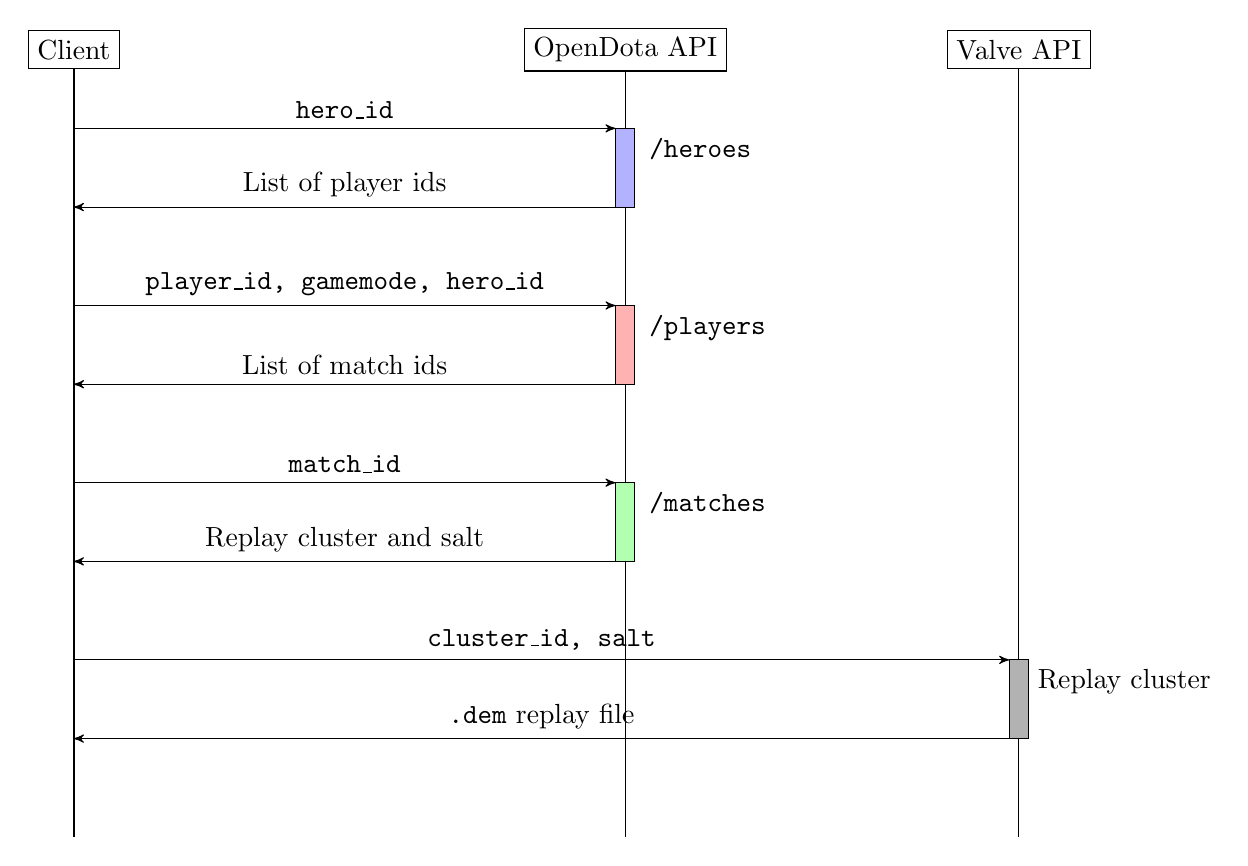
\begin{tikzpicture}[>=stealth']
% Locations
\def\ClientToServer{++(6,0)}
\def\ServerToClient{++(-7,0)}
\def\ValveToClient{++(-12,0)}
\def\Lifeline{++(0,-10)}

% Lifelines
\path (0,0) node[draw] (Client) {Client}
      (7,0) node[draw] (Server) {OpenDota API}
      (12,0) node[draw] (Valve)  {Valve API};
\draw (Client) -- \Lifeline (Server) -- \Lifeline (Valve) -- \Lifeline;

% Blocks
\path (Server)
      ++(0,-1) node (BeginHeroes) {} node[below right] {\texttt{\ /heroes}}
      ++(0,-1) node (EndHeroes)   {};
\filldraw[fill=blue!30] (BeginHeroes.west) rectangle (EndHeroes.east);

\path (Server)
      ++(0,-3.25) node (BeginPlayer) {} node[below right] {\texttt{\ /players}}
      ++(0,-1) node (EndPlayer) {};
\filldraw[fill=red!30] (BeginPlayer.west) rectangle (EndPlayer.east);

\path (Server)
      ++(0,-5.5) node (BeginMatches) {} node[below right] {\texttt{\ /matches}}
      ++(0,-1) node (EndMatches) {};
\filldraw[fill=green!30] (BeginMatches.west) rectangle (EndMatches.east);

\path (Valve)
      ++(0,-7.75) node (BeginReplays) {} node[below right] {\ Replay cluster}
      ++(0,-1) node (EndReplays) {};
\filldraw[fill=black!30] (BeginReplays.west) rectangle (EndReplays.east);


% Calls
\draw[->] (BeginHeroes)\ServerToClient -- node[above] {\texttt{hero\_id}} (BeginHeroes);
\draw[->] (EndHeroes) -- node[above] {List of player ids} \ServerToClient;

\draw[->] (BeginPlayer)\ServerToClient -- node[above] {\texttt{player\_id, gamemode, hero\_id}} (BeginPlayer);
\draw[->] (EndPlayer) -- node[above] {List of match ids} \ServerToClient;

\draw[->] (BeginMatches)\ServerToClient -- node[above] {\texttt{match\_id}} (BeginMatches);
\draw[->] (EndMatches) -- node[above] {Replay cluster and salt} \ServerToClient;

\draw[->] (BeginReplays)\ValveToClient -- node[above] {\texttt{cluster\_id, salt}} (BeginReplays);
\draw[->] (EndReplays) -- node[above] {\texttt{.dem} replay file} \ValveToClient;

\end{tikzpicture}
\caption{Sequence of API calls to download  replay files}
\label{fig:api-calls}
\end{figure}

Figure \ref{fig:api-calls} shows the sequence of API calls that lead to acquiring the replay file from Valve servers. Multiple calls to the OpenDota API is required as each call returns the data needed for the next. This whole process is streamlined as a Node.js script, which takes three parameters: hero id, number of players and number of games per player. Occasionally, the replay files are not found as they may have been deleted, or the cluster unreachable. This is not an issue, as there is a large number of other players and replays that can be downloaded instead. The only implication is the number of replays downloaded may not be the exact number of replays specified (number of players $\times$ number of games per player).

\subsubsection{Data processing}
The data processing is done using the parser \texttt{clarity} \cite{clarity}. It is an open source tool developed by Martin Schrodt that parses and extracts in game data from a replay file. The overwhelming amount of data available in a single game means the parser acts as an interface to access any entity or combat log. In some cases, the data is provided as an original protobuf object. The data gathered is output as a csv. For the forensic mouse movements, each row represents a level 3 action, giving thousands of level 3 actions for every game. On the other hand, there is only one set of game-specific features for each game, so there is only one row of game-specific features for each game. 


\subsubsection{Feature extraction}
With the csv data available after parsing, the data is collated into \texttt{pandas} Dataframes using Python. The dataframes provide many useful functions, such as dealing with NaNs and merging dataframes together. The dataframes are also match perfectly with the \texttt{scikit-learn} machine learning library in Python, which is able to take in any dataframe as input, treating each row of the dataframe as a data point for training. 

The features extracted into the dataframes differ depending on the machine learning model and problem. For some models, the dataframes were unchanged from the raw csvs, but for others, further processing was done. For more complex models which require further processing of dataframes, the resulting dataframes are stored in order to reduce the time taken so the dataframes do not have to be re-calculated and created when new models or techniques are trained and tested. 


\subsection{Predicting the player (Game classification)}
The first machine learning problem was modelled as a binary classification problem. The model was trained on the question: \textit{Given a game of Dota 2, is the player on a specific hero the player we are looking for?} The problem used a fixed hero in order to remove any extra complexity that may rise from including different heroes, such as playstyle of the hero. 


\subsubsection{Methodology}
This problem was investigated with two different uses of the data.  Initially, each individual level 3 action was taken as a single data point for training, rather than all level 3 actions in a single game. This meant there was no concept of a game, as the model simply took lists of level 3 actions instead. The three level 3 actions were each used individually to see which would be more indicative for identifying the player. In this sense, it be asking the question: \textit{Given a level 3 action, is the player who performed this action the player we are looking for?} Each action was assigned as a positive sample if came from the particular player, and a negative sample otherwise. This meant there was a large number of training and testing samples, as each game contained thousands of level 3 actions. Further, the mouse movement features and game-specific features were investigated independently in order to see how effective each type of feature. Clearly, this is not a very realistic experiment or result to look at, but it gives a good indication that looking at mouse movements alone can have some amount of predictive capabilities. 

In the second iteration of this problem, the level 3 actions were combined together so that a model could be trained on individual games as data points rather than actions. In this approach, a separate model was used for each of the level 3 actions as before, but the results of the models are combined by a simple voting mechanism and a simple MLP classifier. This gave a better representation of identifying a player from a game from training, rather than a large list of level 3 actions. This time, a more rigorous approach was used, making sure games from the training data did not appear in the testing data. Further, the same method was applied to different heroes and players. This showed the model being general enough to work for any hero or player as long as it was re-trained. 

%\begin{figure}[H]
%\caption{Difference between the first and second approach towards mouse movements in game classification.}
%\end{figure}

%\subsubsection{Results}
%TODO graphs



\subsection{Predicting the same player (Pair classification)}
There was a subtle issue with the way the first binary classification problem was framed, which led to very good accuracy and results for the machine learning model. The issue is that the first problem only worked and trained on a fixed set of players, and predicted out of that fixed set, whether it was one of the players or not. In the first stages, when testing on a small set of ~10 players, this gave very good results as the model only had to predict if a game belonged to one of the ten players. This meant that the model was not generalisable the set of every Dota 2 player, as it is not possible to train on all games by every player. Most importantly, the model is not able to predict games by players it has not trained on, always being fixed to the set of players used in training. To confirm this was an issue, the same model was trained and tested on a much larger set of players. It would be expected that the accuracy be reduced with an increased set of unique players, as the model must predict one player out of a larger pool.

To solve this issue, the problem was framed in a different way. Rather than ask, \textit{Given a game, which player does it belong to?}, the problem is framed as \textit{Given a pair of games, do they both belong to the same player?}. This question is subtly different, as the goal is to train on a large mix of players and games, then to be able to predict whether two games belong to the same player, even if that player has never been seen before in training. Moreover, this can be extended such that \textit{Given a game and a player id, does the game belong to that player?} by applying the pair problem for a list of games from the player id. The idea is instead of finding a pattern for a specific player based on the features, which would not be general, the model finds a pattern to differentiate two players given two sets of the features for comparison. 

\subsubsection{Methodology}
The mouse movement features were altered from the game classifier problem in order to fit into this problem. Before, each game was evaluated separately, so every level 3 action could be used. However, in this pair problem, two games must be used as inputs to the model. As games are of different lengths, the number of level 3 actions will be different for every game, which prevents the model taking every level 3 action as input. Instead, statistics such as the average, standard deviation and range are used for the list of level 3 actions over the entire game. This causes lots of data to be lost, as the hundreds of level 3 actions are reduced to a few statistics. To alleviate this issue as much as possible, the games are split into portions, where each portions has its own statistics. For example, each game can be split into thirds where each third will have its own average and standard deviation for each type of level 3 action. Splitting a game like this not only decreases the data loss due to averaging, but enables each portion to be evaluated individually to see whether any section of a game is more indicative of player behaviour compared to another section. 



\section{Conclusion and future work}
A lot of the foundational work has been completed, and a working model and machine learning pipeline have been established with good results. The goal of the next few weeks is to discover how to improve on the current results and find interesting relationships between the data and the predictive power of the models. 

\subsection{Additional game-specific features}
Although there are some game-specific features used in the current models, there are some more strategy-based features that can be easily extracted. These are features such as item purchases, skill builds and item slots. These features are potentially very useful, as players have different strategies and preferences for certain items or builds. At the same time, the same strategy can often be echoed by a majority of players because it is the most optimised and established strategy. Regardless, it is important to include these features as it is interesting to see whether they are useful or not, especially depending on the combination of these features with the other features that have already been extracted. 

\subsection{Graphs and results}
All results gathered so far in the project are preliminary results used to guide the direction of the project. The results are a means to get an early indication as to the success of the various approaches used. However, because they have not been gathered through a methodical method, it is currently difficult to draw comparisons between the different models and experiments. Going forward, an important step is to establish a method in which all models can be evaluated against, using the same data.

\subsection{Pair classification with account ids}
Though the current models are able to perform classification on a pair of games, ideally  they take a single game and an account id. This can be done by downloading more games from the given account id and running a pair classification on each downloaded game and the given game. 

Another point of concern is that currently all machine learning has been done using the a fixed hero. This removes the additional factor of hero selection affecting the results and features, as different heroes have different playstyles. It is still under discussion whether to start the major piece of work to incorporate hero selection as part of the pipeline, rather than excluding it. A simpler solution would be to train a different model for each hero. This means the models will not be general to all heroes, but could be interesting to see if some heroes are more predictive than others, or whether some heroes need tweaked models. 

\subsection{Feature selection}
There are many known methods and algorithms that can be used to select a subset of features for machine learning. The current method of feature selection is based on heuristic knowledge of what might be useful, but it is difficult to judge especially when it comes to the combination of many features. It would be interesting to see what the best results can be achieved by heuristic selection of features, and compared these results to those achieved by automatic selection algorithms. Perhaps the feature selection algorithms can pick out combinations that give good results and remove noise that would not have been thought of from a heuristic point of view. 

\printbibliography

\end{document}
